\chapter{Experiments with Real Data}
\section{Equipment Setup and Data Collection}
In order to examine the accuracy and feasibility of the algorithm
being used in low flying UAV for obstacle detection purpose, realistic
aerial video and navigation data are collected through a test flight
with the support of Sander Geophysics Ltd. A main purpose of the test
flight is to obtain a piece of aerial video with the camera close to
the ground as much as possible. This is difficult to achieve with any
manned fixed wing aircraft. Therefore, a simulated unmanned aircraft
system (SUAS) was used to carry all sensors. The SUAS is then towed by
a helicopter via a tow rope of 33 meters long (Figure
\ref{fig:towedSUAS})to complete the survey. Yet, to prevent the SUAS
from being caught by tree top, sufficient clearance must be left
between the SUAS and the vegetation. As a result, the helicopter flew
a planned path at approximately 100 meters above ground, and SUAS at
approximately 70 meters above ground.

\begin{figure}[h]
\centering
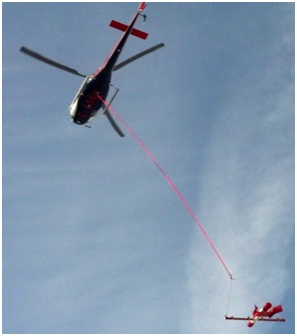
\includegraphics[width=7.75cm,keepaspectratio=true]{./Figures/towed_SUAS.jpg}
\caption{Simulated UAS towed by helicopter}
\label{fig:towedSUAS}
\end{figure}

Sensors mounted on the SUAS included one wide angle CCD camera with 6
mm focal length lens capturing monocular image sequence at 30 fps, a
pair of narrow angle CCD cameras for binocular images, one GPS
antenna, and one flight control INS/GPS navigation unit Athena GS-111m
\cite{_athena_????}(Figure \ref{fig:SUAS}). Analog video and
navigation data are sent to the helicopter via three BNC cables and
one data cable. Installed in the helicopter are two SGL data
acquisition system CDAC. This system records video and data from SUAS,
as well as data from sensors installed on the helicopter, including
GPS, radar and laser altimeter, air pressure, temperature, humility,
etc. Navigation data from the SUAS were sent in RS485, and were
directly recorded via the UART port of the computer (figure
\ref{fig:CDAC}). Videos from the three cameras were digitized to
720x480 resolution images using a PC/104+ MPEG4 video encoder from
Parvus installed in CDAC. The video were time-stamped with GPS second
on the image screen for post-flight synchronization with the
navigation measurements. A snapshot of the digitized video is shown in
figure \ref{fig:video_snapshot}.

\begin{figure}[h]
  \centering
  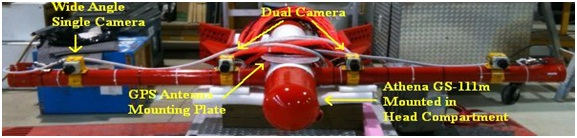
\includegraphics[width=14cm,keepaspectratio=true]{./Figures/SUAS.jpg}
  \includegraphics[width=6cm,keepaspectratio=true]{./Figures/athena.jpg}
  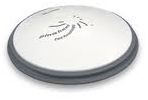
\includegraphics[width=6cm,keepaspectratio=true]{./Figures/GPS_antenna.jpg}
  \caption{Sensors mounted on SUAS. Top: the SUAS, bottom left: Athena
  GS-111m, bottom right: GPS antenna}
  \label{fig:SUAS}
\end{figure}

\begin{figure}[h]
  \centering
  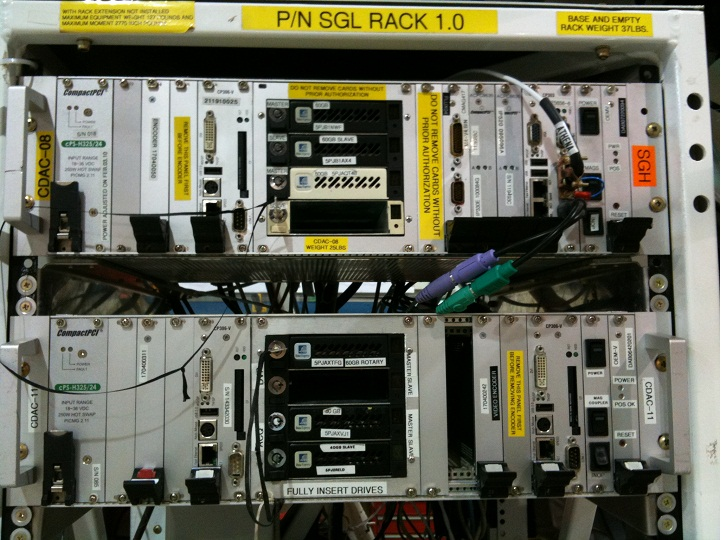
\includegraphics[width=12cm,keepaspectratio=true]{./Figures/CDAC_Rack.jpg}
  \caption{Compact PCI data acquisition system (CDAC)}
  \label{fig:CDAC}
\end{figure}

\begin{figure}[h]
  \centering
  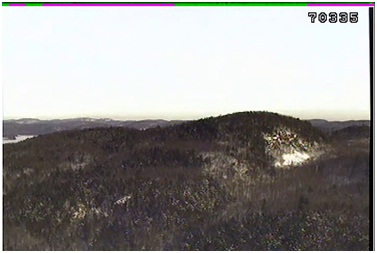
\includegraphics[width=12cm,keepaspectratio=true]{./Figures/video_snapshot.jpg}
  \caption{Image from monocular camera with GPS second timestamp}
  \label{fig:video_snapshot}
\end{figure}

\section{Camera Calibration}

A camera calibration was performed after the flight by taking a piece
of video of a checker board pattern with various translation and
rotation motion. A total of 20 views of the calibration target was
chosen from the video, and fed to the calibration algorithm. A few
examples were shown in figure \ref{fig:camcal}. The
algorithm,``calibration.exe'', used for calibrating the camera comes
with the OpenCV installation. Table \ref{tab:calresult} below listed
the calibration results.

\begin{center}
\begin{tabular}{|c|c|}
\hline
Image Width & 720 pixels \\ \hline
Image height & 480 pixels\\ \hline
$f_x$ & 887.6\\ \hline
$f_y$ & 805.7\\ \hline
$c_x$ & 381.8 \\ \hline
$c_y$ & 293.7 \\ \hline
$k_1$ & -0.102 \\ \hline
$k_2$ & -0.535 \\ \hline
$p_1$ & 1.15e-003 \\ \hline
$p_2$ & 8.40e-003 \\
\hline
\end{tabular}
\end{center}

\section{Ground Truth Data Collection and Comparison}

UAS localization ground truth are obtained through onboard flight
control unit GS-111m. The unit records the SUAS position in GPS
longitude and latitude coordinate. Orientation is obtained from the
roll pitch and heading measurements. Roll and pitch accuracy has
$0.1^\circ$ mean and $0.1^\circ$ standard deviation. Heading accuracy can
achieve $0.5^\circ$.\cite{_athena_????}

The estimated SUAS position can be directly obtained from the inverse
of world origin estimation in the CC\_EKF\_SLAM state vector:
$[O_{XYZ}^{c}, W_{XYZ}^{c}]$.

Digital elevation map (DEM) are downloaded from CGIAR-CSI website
\cite{_cgiar-csi_????} and used as ground truth data for feature
mapping. The downloaded DEM contains longitude, latitude and see level
elevation of the terrain with a resolution approximately 100 meters by
100 meters. To compare estimated feature position to the the DEM, some
conversion are necessary to bring both data to the same coordinate
system. In this work, the comparison are done in UTM coordinate. 

First, the longitude and latitude in DEM data are converted into UTM
using the WGS84 world geodetic system \cite{_world_????}. Many library
are readily available to do the conversion by taking GPS coordinate
and zone number as input. The library used in this work is a python
interface to PROJ.4 library \cite{_pyproj_????} called pyproj
\cite{_pyproj_????}. Secondly, the DEM data in UTM were converted into
world frame using transformation matrix with intial SUAS position and
orientation as input.

To bring result from the CC\_EKF\_SLAM algorithm to world frame, feature
coordinates must be first converted into world frame using the
estimated UAS localization results. Let $[X_i^W,Y_i^W, Z_i^W]^T$ be
the feature coordinate in world frame, it can be calculated by

\begin{equation}
  \left[ \begin{array}{c}
    X_{i}^{W}  \\
    Y_{i}^{W}  \\
    Z_{i}^{W}  \\
  \end{array} \right]=Q^{-1}(O_{XYZ}^{c}, W_{XYZ}^{c})\left(\left[
    \begin{array}{c}
      x_{i}^{C} \\
      y_{i}^{C} \\
      z_{i}^{C} \\
    \end{array}
  \right]+\frac{1}{\rho _{i}}m(\varphi _{i}^{C},\theta_{i}^{C})\right)
\end{equation}

%%% Local Variables:
%%% mode: latex
%%% TeX-master: "thesis.tex"
%%% End:
